\section{Multi-GPUs algorithm} \label{multi_GPU}
\subsection{Domain decomposition}

While a single GPU has demonstrated commendable performance in numerous applications, the computational demands entailed in simulating extensive more large-scale problems surpass the capabilities of a single GPU. It is necessary to explore the development of parallelization techniques using multiple GPUs to address this issue. For descriptive convenience, our multiple-GPU algorithm is presented using a two-dimensional grid as a paradigm, with the situation for three-dimensional grids being analogous.

Our study employs the domain decomposition method to partition a 2D grid with $Nx \times Ny$ dimensions into $m$ parts along the $x-$coordinate direction. Each part represents a sub-domain; the total number of sub-domains is denoted as $m, m$ equals the total number of GPUs in use. Each sub-domain is assigned to a corresponding process equipped with a GPU for computation. Throughout the simulation, the variables of each sub-domain persistently reside in the global memory of the assigned GPU.
\begin{figure}[ht]
    \centering{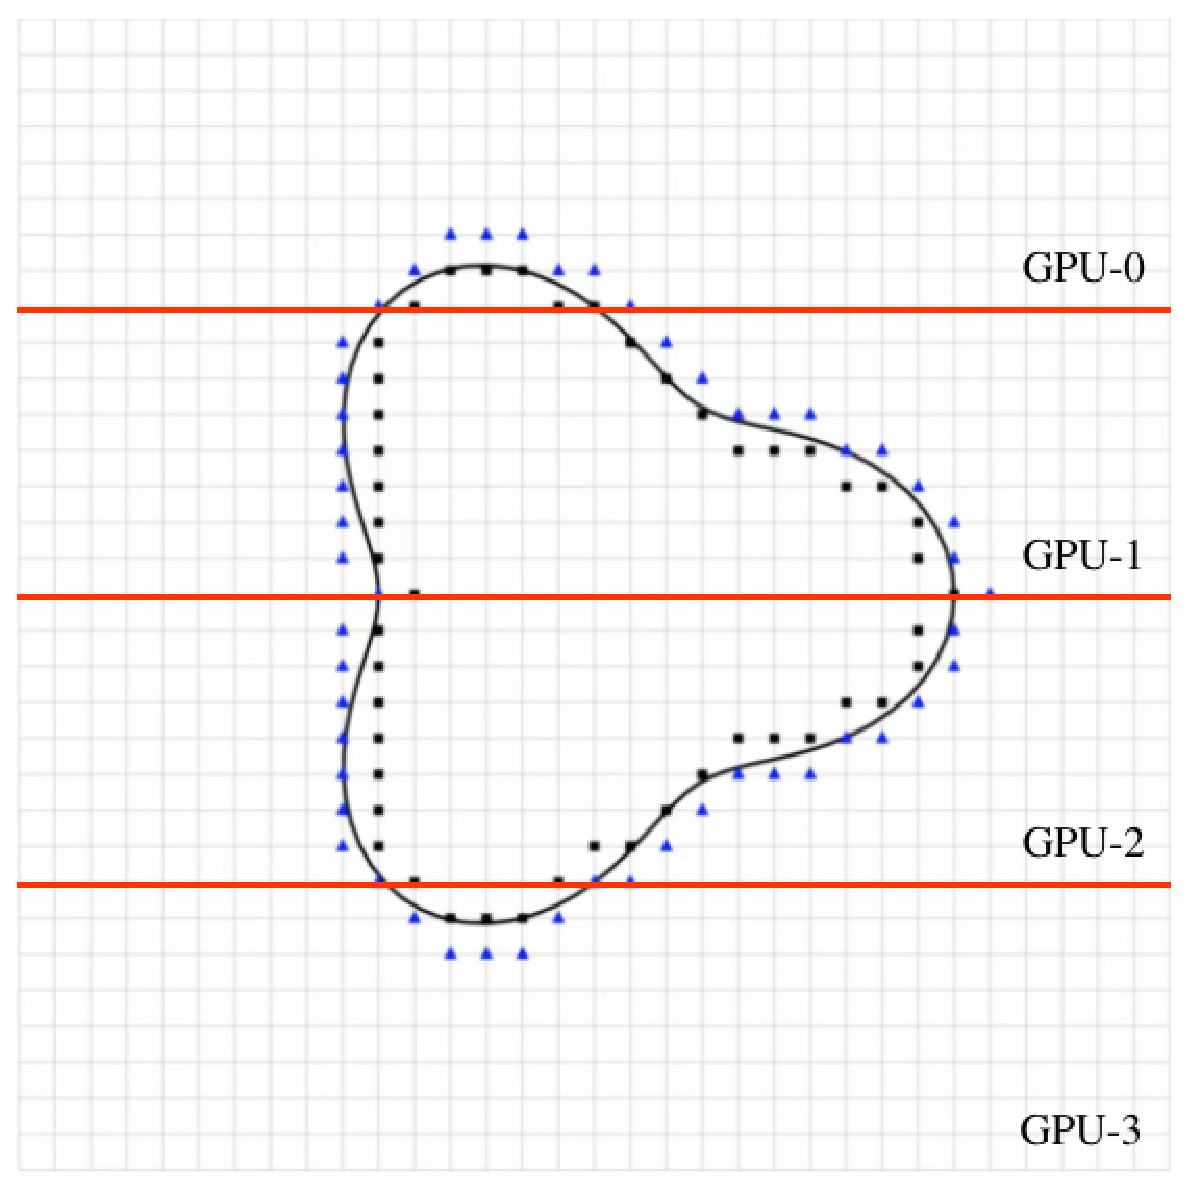
\includegraphics[width=0.4\textwidth]{figure/one_gpu_irregularNode2.eps}}
    \caption{Partition the Cartesian grid into four subdomains along the y-axis, with each subdomain assigned to a dedicated process equipped with a GPU for computation.}
\end{figure}

In the interface problem-solving process, each process stores the relevant information of curve points within its allocated region. Initially, all the data points on the boundary are gathered to calculate the solutions at these specific curve points. Subsequently, the computed results are distributed back to the respective processes.

Before set up the iteration in Section \ref{one_GPU:solver}, the CPU's grid data and boundary data are distributed to their respective processes based on regions. Subsequently, this data is efficiently copied to the device. Throughout the iterative solving process, each process is responsible for processing the pertinent information related to grid points, control points, and intersection nodes within its designated region, and all computations are carried out on the GPU. Upon completion of the iteration, the processed data is then returned to the host system. This approach ensures a standardized and optimized procedure for utilizing CUDA-enabled devices to expedite the solving process.

\subsection{Data communication}
\begin{figure}[ht]
    \centering{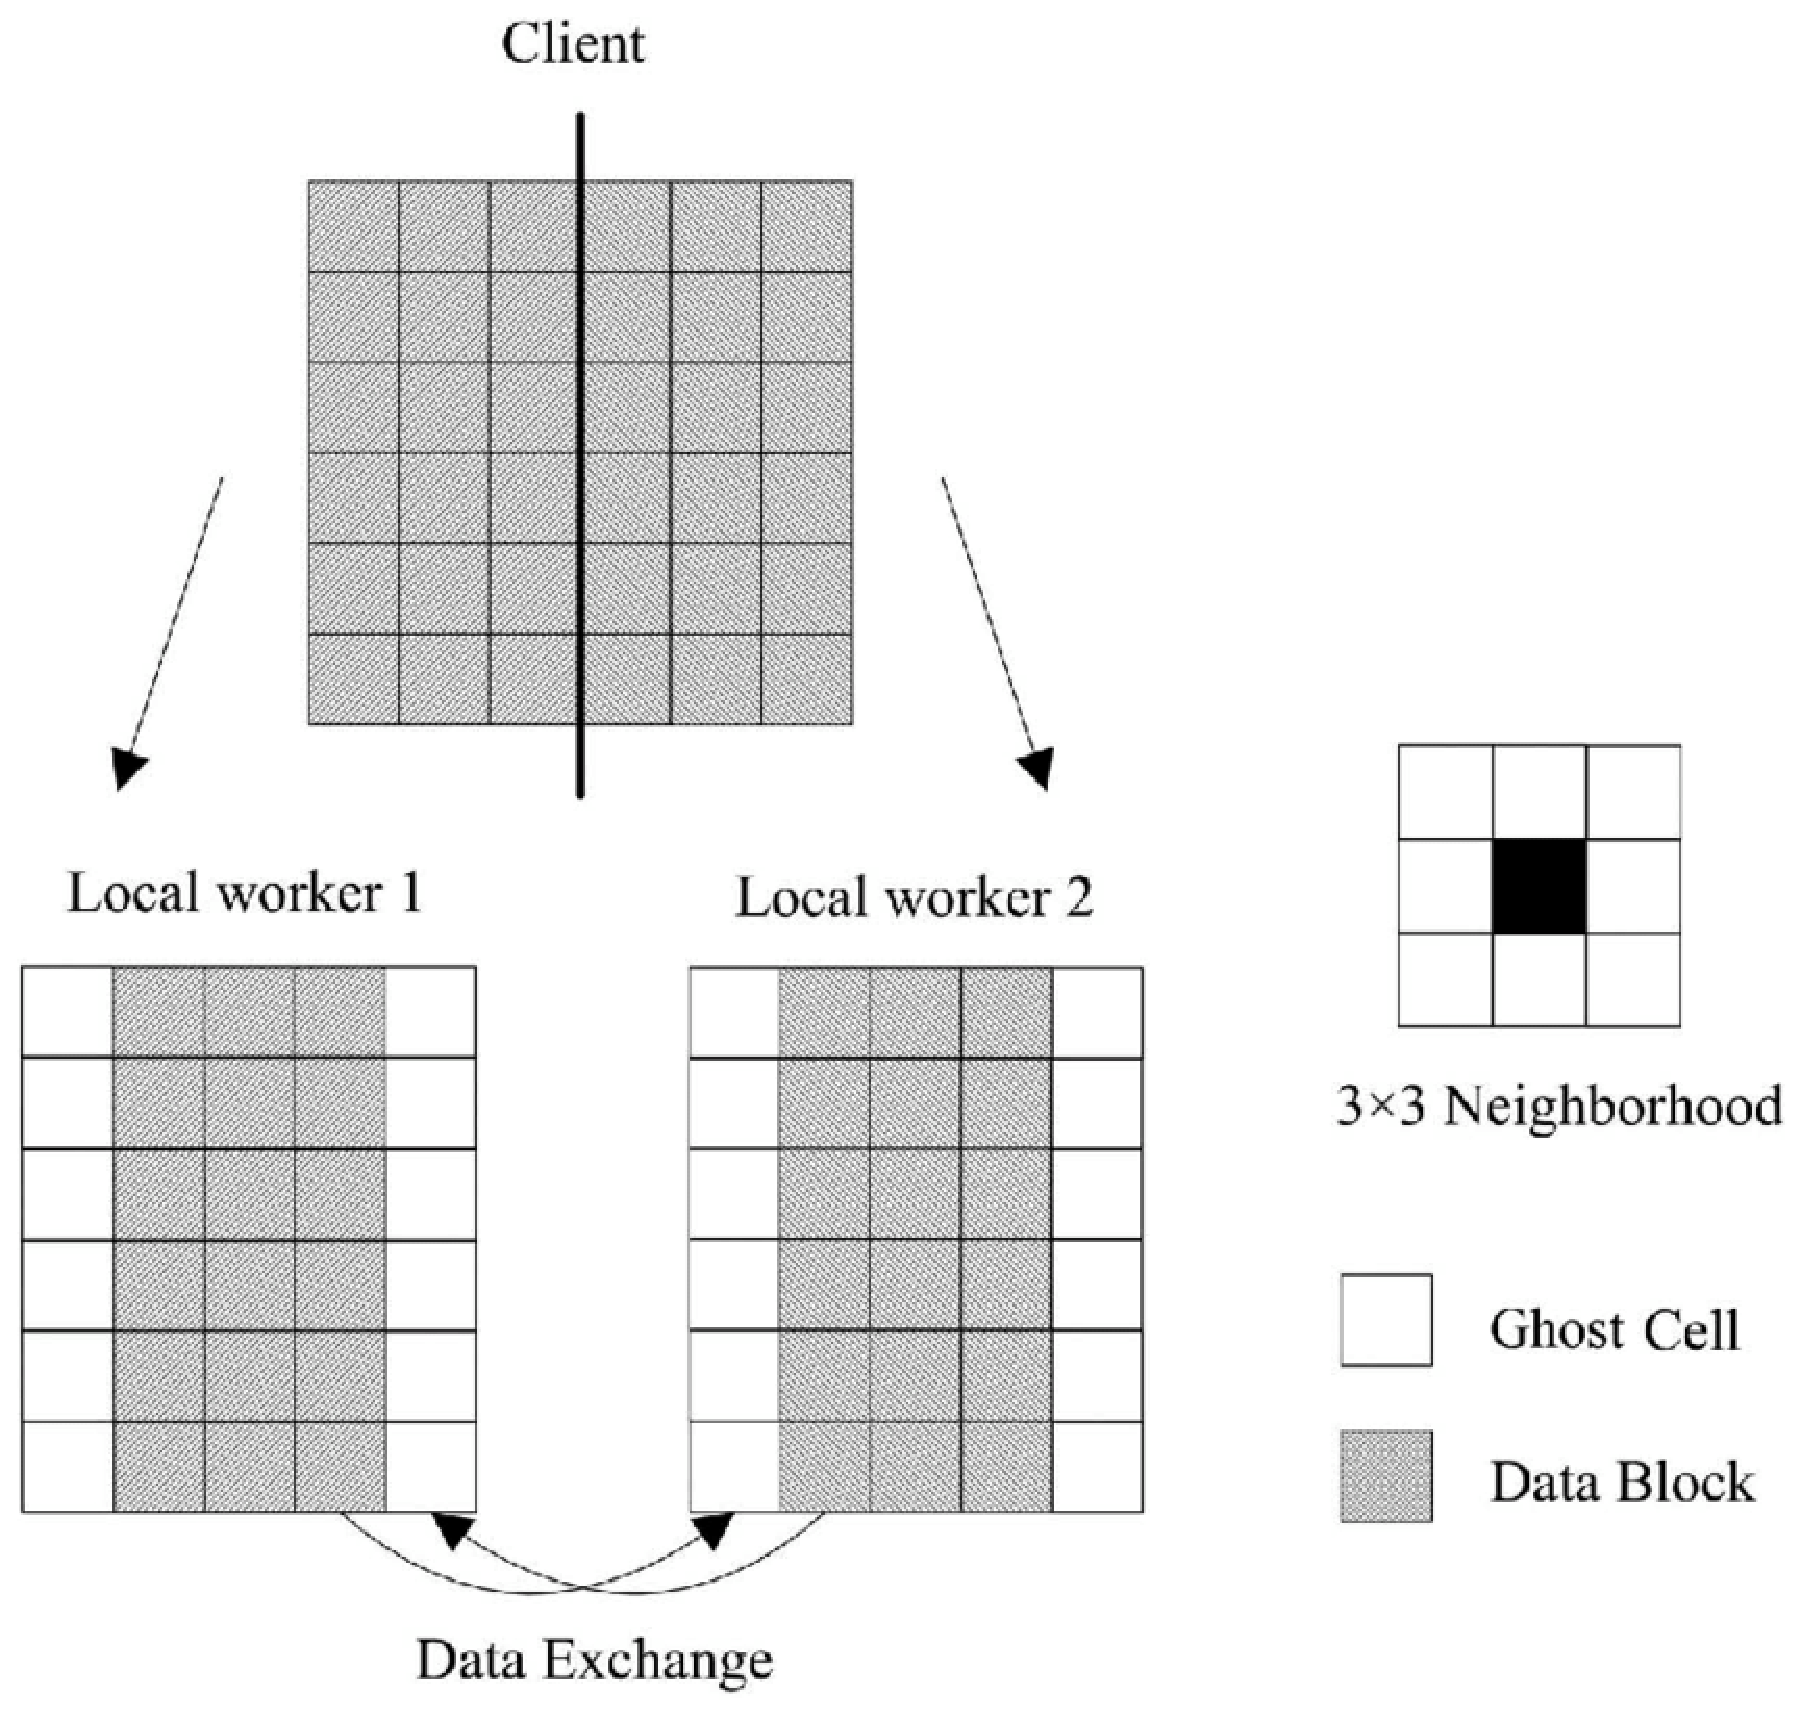
\includegraphics[width=0.4\textwidth]{figure/ghost3.eps}}
    \caption{Each process is accompanied by a peripheral layer of a virtual subdomain, situated at the boundaries of their respective regions, which serves the purpose of receiving boundary data transmitted by neighboring processes.}
 	 	%	\label{125000}
\end{figure}

In order to facilitate efficient data exchange, MPI is utilized on the CPU to transfer data from two layers of internal units adjacent to subdomain boundaries. We allocate memory spaces on both the host and the device to store secondary boundary data. Once the boundary of a specific subdomain is computed, each device uploads the necessary boundary data to the virtual region, which is then downloaded by neighbouring devices to prepare for the subsequent computational steps. This approach optimizes data exchange while minimizing data redundancy between the CPU and GPU.

Given that there are fewer control points than grid points, the time and computational cost associated with collecting and disseminating potential values, denoted as $\phi$ and $\psi$, across various boundary regions is relatively low. During the process of solving the interface problem \eqref{one_GPU:interface}, each process is tasked with obtaining potential function information for all control points. To streamline this procedure, MPI is employed to consolidate the potential function information before the interface problem calculation begins. Upon completion of the calculation, MPI is once again used to distribute the results back to their respective processes. 
\subsection{Poisson solver}\label{distribute Poisson}
% \subsubsection{Algorithm}
% For the Poisson equation, we employ a three-step process to solve the modified linear system:
% \begin{enumerate}
% \item  FFT in $x$-direction: Firstly, the data is transformed by FFT. This operation is performed in the $y$ direction, and the Fourier coefficients are computed using the CUFFT library. This step allows for efficient manipulation of the data in the frequency domain.
% \item Distributed Arrowhead Decomposition method: Next, we utilize a distributed arrowhead decomposition method to decompose the tridiagonal linear system in the $x$ direction. This technique facilitates solving the linear tridiagonal equations for each sub-domain on the corresponding GPU. We leverage the cusparseDgtsv2StridedBatch API from the CUSPARSE library for an efficient and accurate solution of the linear equations.
% \item IFFT in $x$-direction: Finally, the data is transformed back to the spatial domain using the inverse fast Fourier transform. This operation is performed in the $y$ direction, and the Fourier coefficients are calculated once again using the CUFFT library. This step allows us to obtain the final solution of the Poisson equation.
% \end{enumerate}
For the FFT-based solver of the Poisson equation, we still follow the process Algorithm \ref{one_GPU:FFT_algo}. Unlike single GPU, we solve tridiagonal linear equations using the distributed arrowhead decomposition method(ADM)\cite{arrowhead2017}. The ADM is an efficient algorithm, and the resulting system is suited for designing distributed algorithms for each sub-domain on the corresponding GPU.

\subsubsection{Arrowhead decomposition method}
The linear equation system to be solved is denoted as : $Au = f$.
\begin{figure}[htb]
    \centering
    \subfigure[Intial linear system]{
	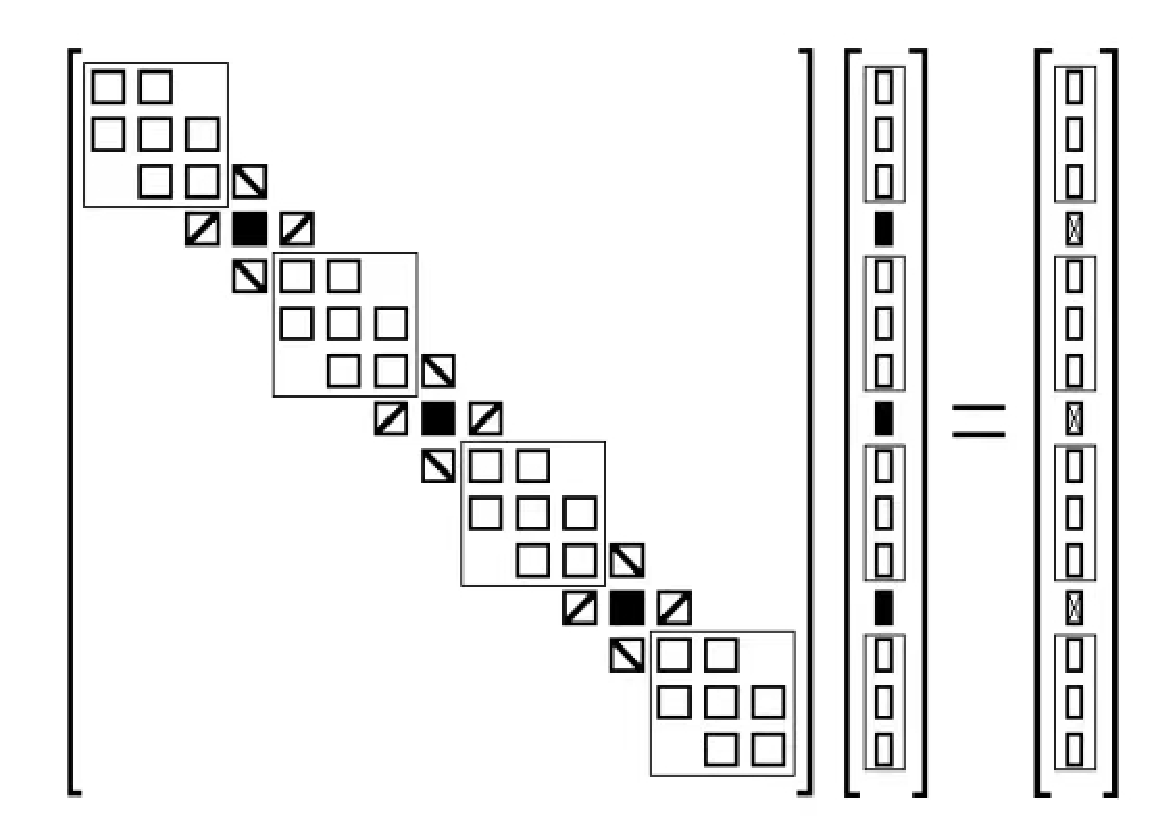
\includegraphics[width=0.3\textwidth]{figure/triangleM_a.eps}
	\label{fig:multi_GPU:triangle_a}
    }
    \subfigure[Rearranged linear system]{
   	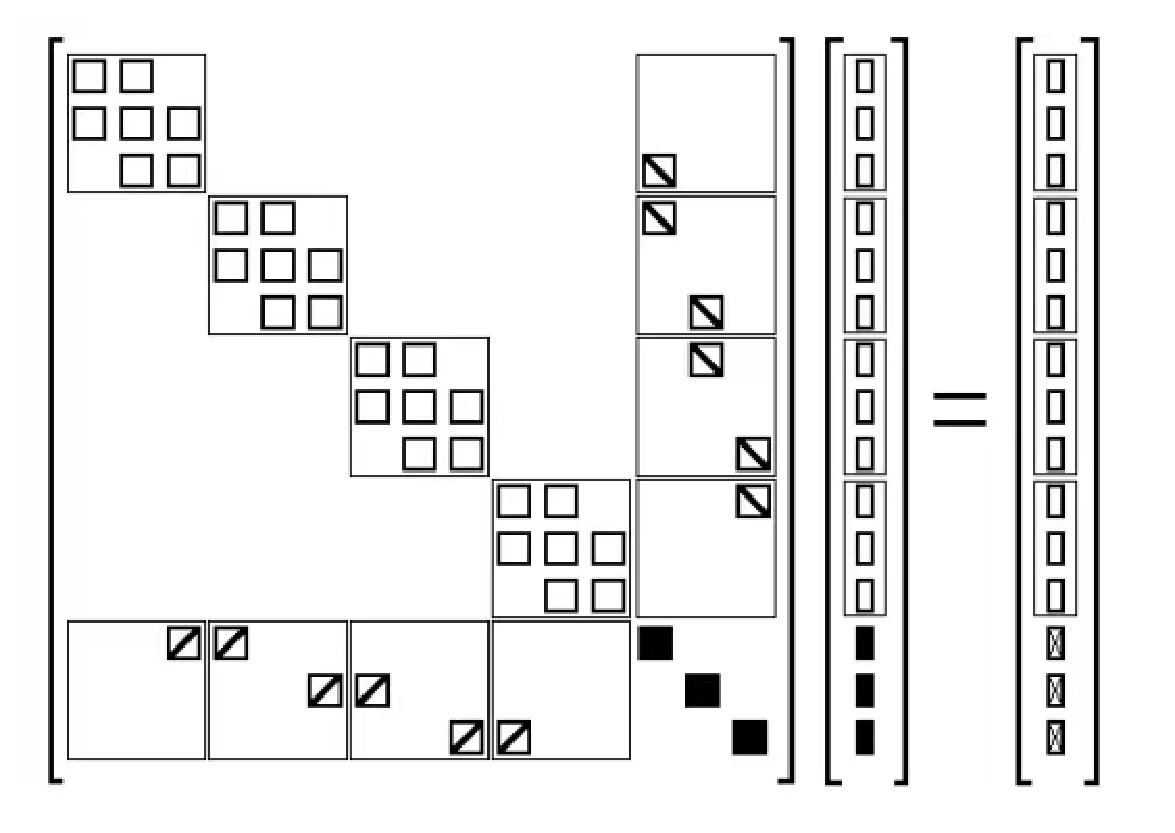
\includegraphics[width=0.3\textwidth]{figure/triangleM_b.eps}
	\label{fig:multi_GPU:triangle_b}
    }
    \subfigure[Notation of the rearranged system]{
   	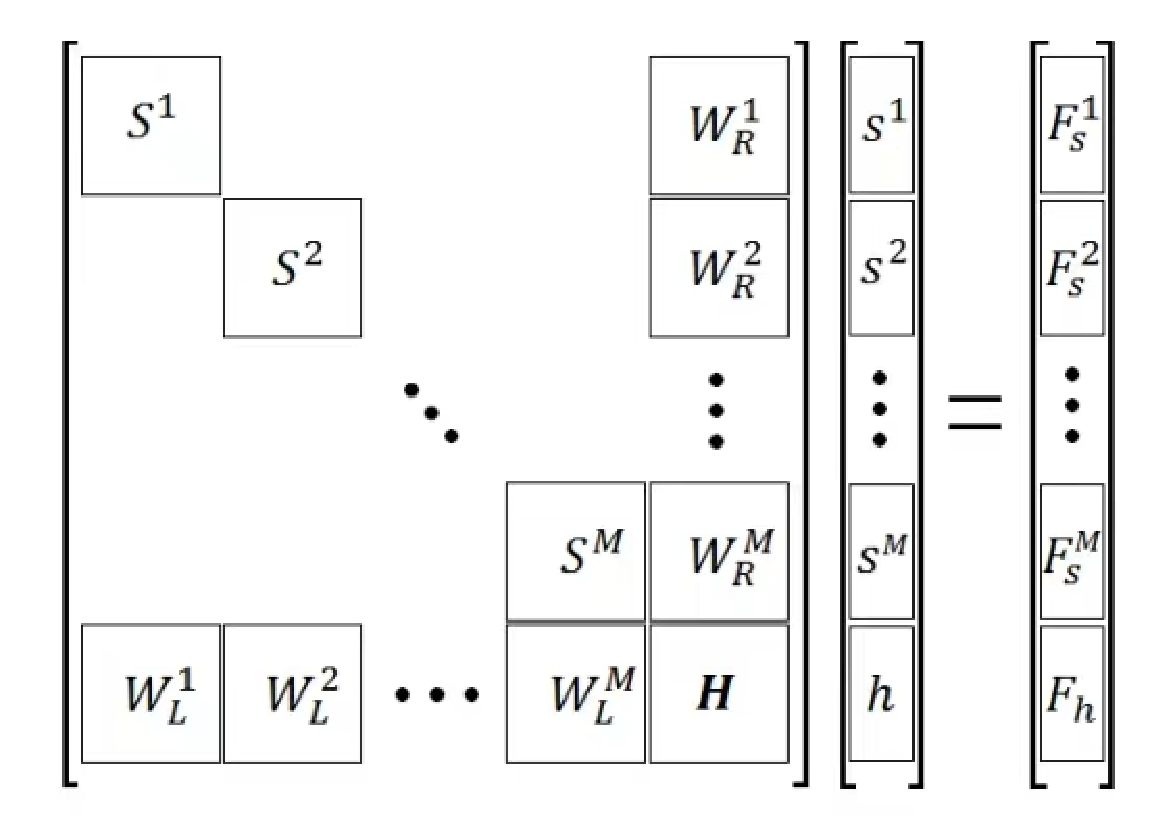
\includegraphics[width=0.3\textwidth]{figure/triangleM_c.eps}
	\label{fig:multi_GPU:triangle_c}
    }
    \caption{A graphical scheme for rearrangement of the initial block-tridiagonal linear system into the equivalent form, coming from \cite{arrowhead2017}. Left: the initial matrix $A$ with blocks. Center: after rearrangement, the initial matrix becomes "arrowhead" matrix. Right: the denotation of the "arrowhead" matrix.}
    \label{Schur Complement Method}
\end{figure}
Fig.\ref{Schur Complement Method} depicts the concept of ADM. A similarity transformation transforms the initial block-tridiagonal linear system\eqref{block-tridiagonal} into an equivalent block matrix form. This reorganization is particularly advantageous for region decomposition and the design of distributed algorithms, as each block matrix's linear system exhibits a degree of independence. The reordering is carried out by exchanging block rows and block columns, which, in turn, affects the elements of the unknown vector and the right-hand side vector. The resulting matrix structure can be represented as a $2 \times 2$ block matrix.
\begin{equation}
\left(\begin{array}{cc}
\mathbf{S} & \mathbf{W}_R \\
\mathbf{W}_L & \mathbf{H}
\end{array}\right)\left(\begin{array}{l}
s \\
h
\end{array}\right)=\left(\begin{array}{l}
F_s \\
F_h
\end{array}\right)
\label{block-tridiagonal}
\end{equation}

In this context, the unknown solution vector $h$ corresponds to the movable component of the complete solution, as illustrated in Figure \ref{Schur Complement Method}. The square super-block $\mathbf{S}$ comprises new independent tridiagonal blocks $S^k$, with $k=1, \ldots, M$, positioned along the diagonal. The matrix elements $\mathbf{H}$ form the lower-right coupled super-block, representing the coupling of unknowns at the interface. Additionally, the other horizontal super-blocks $\mathbf{W}_R$ and $\mathbf{W}_L$ are supplementary components within the matrix, signifying the internal unknowns of the coupling processors at the interface. The following relationships determine the solution of the system\eqref{block-tridiagonal}.

\begin{equation}
\left\{\begin{array}{l}
s=\mathbf{S}^{-1} F_s-\mathbf{S}^{-1} \mathbf{W}_R h \\
h=\left(\mathbf{H}-\mathbf{W}_L \mathbf{S}^{-1} \mathbf{W}_R\right)^{-1}\left(F_h-\mathbf{W}_L \mathbf{S}^{-1} F_s\right)
\end{array}\right.
\label{block-tridiagonal:schur}
\end{equation}

These relationships involve matrix products and inversions, which can be parallelized to a certain extent. The independence of blocks $S^k$ allows for distributed parallel computation of the products $\mathbf{S}^{-1} F_s$. In practice, rather than computing inversions, we efficiently solve the distributed linear systems $Sx = F_s$ due to the special properties of $S^k$. The sparse structure of $\mathbf{W}_L$ and $\mathbf{W}_R$ significantly reduces the number of matrix operations in\eqref{block-tridiagonal:schur}. Once a portion of the total solution $\mathbf{X}=(s, h)^T$ is obtained from the second relationship in\eqref{block-tridiagonal:schur}, i.e., $h=\left(h^1, \ldots, h^{M-1}\right)^T$, the remaining parts can be computed in parallel over GPU $k$ using the provided formula.
\begin{equation}
s^k=z^k-Z^k h^{k-1}-Z^k h^k
\label{trans}
\end{equation}
where formally $z^k=\left(S^k\right)^{-1} F_s, Z^k=\left(S^k\right)^{-1} W_R^k$, and $h^0=h^M=0$.

% \begin{figure}[H]
%  	 		\centering
%  	 		{
%  	 			\includegraphics[width=0.7\textwidth]{figure/trianglematrix.png}
%  	 		}
%  	 		\centering
%     \caption{A graphical scheme for rearrangement of the initial block-tridiagonal linear system
% into the equivalent form.}
%     \label{Schur Complement Method}
%  	 	%	\label{125000}
% \end{figure}

% \begin{figure}[htb]
%     \centering
%     \subfigure[Intial linear system]{
% 	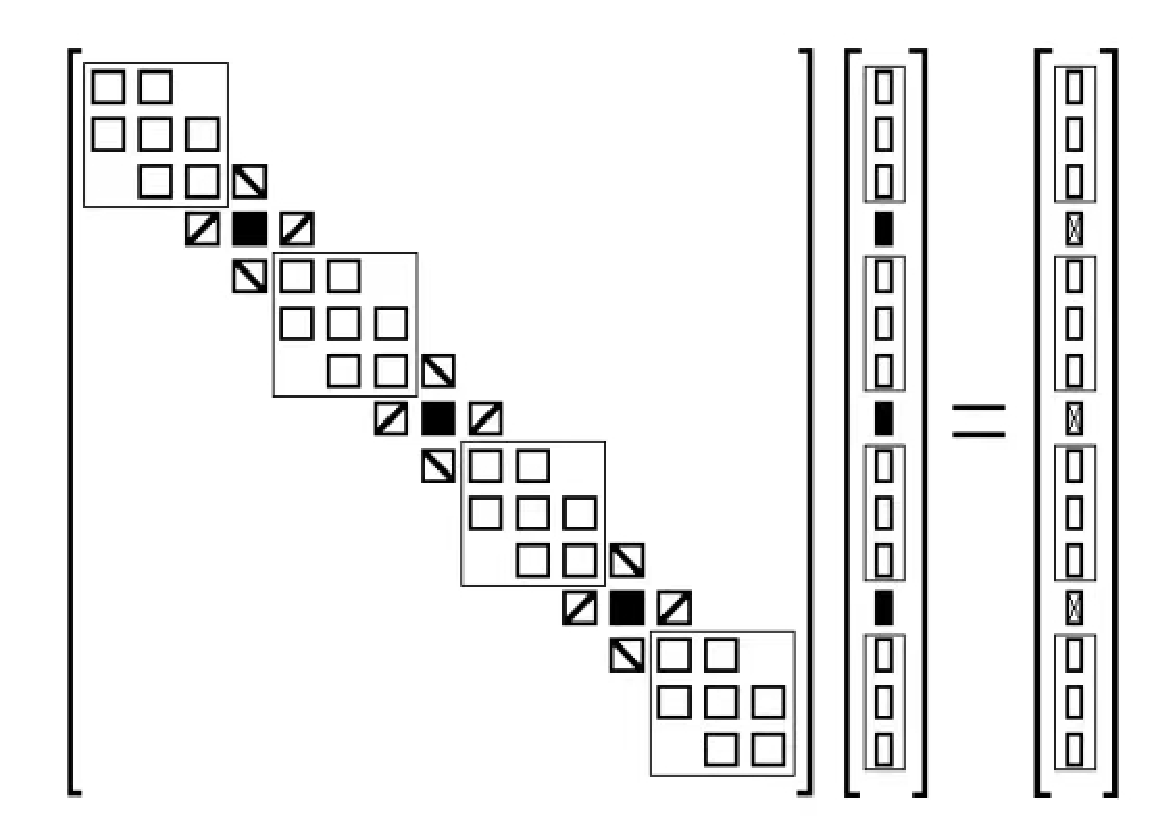
\includegraphics[width=0.3\textwidth]{figure/triangleM_a.eps}
% 	\label{fig:multi_GPU:triangle_a}
%     }
%     \subfigure[Rearranged linear system]{
%    	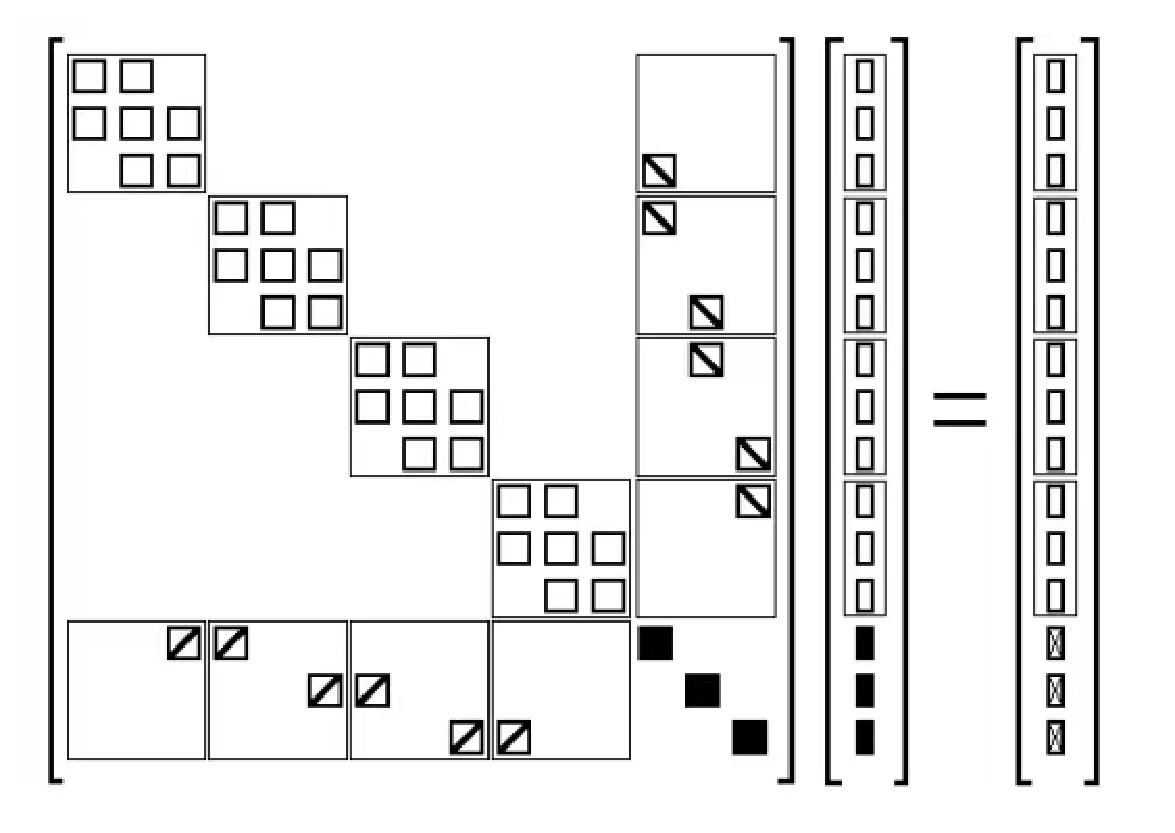
\includegraphics[width=0.3\textwidth]{figure/triangleM_b.eps}
% 	\label{fig:multi_GPU:triangle_b}
%     }
%     \subfigure[Notation of the rearranged system]{
%    	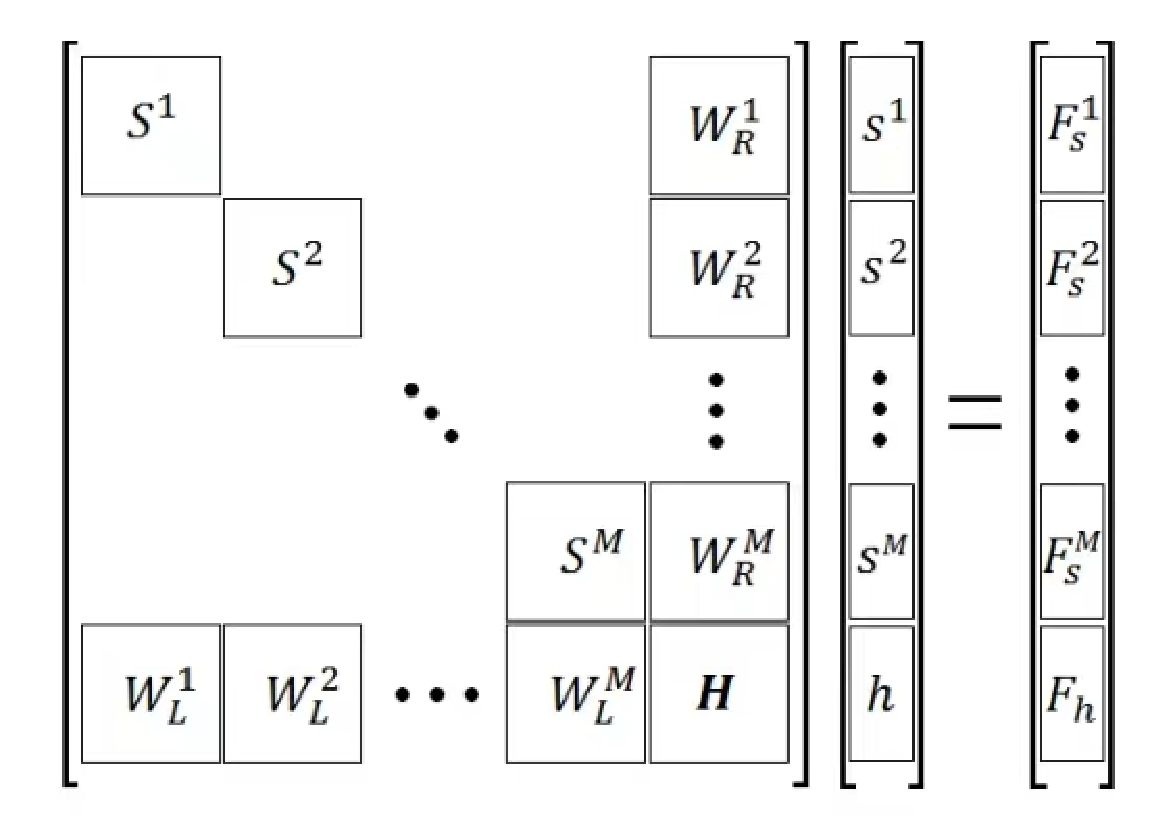
\includegraphics[width=0.3\textwidth]{figure/triangleM_c.eps}
% 	\label{fig:multi_GPU:triangle_c}
%     }
%     \caption{A graphical scheme for rearrangement of the initial block-tridiagonal linear system into the equivalent form, coming from \cite{arrowhead2017}. Left: the initial matrix $A$ with blocks. Center: after rearrangement, the initial matrix becomes "arrowhead" matrix. Right: the denotation of the "arrowhead" matrix.}
%     \label{Schur Complement Method}
% \end{figure}

The distributed algorithm for solving tridiagonal matrices can be outlined as follows:
\begin{algorithm}[H]
\renewcommand{\algorithmicrequire}{\textbf{Input:}}
\renewcommand{\algorithmicensure}{\textbf{Output:}}
\caption{Distributed solver for arrowhead decomposition method}
\begin{algorithmic}[1]
\Require $\text{corrected value} ~\tilde{f}_{i,j}$ and known matrix $A$.
\Ensure $\text{the solution of}$ $Au = f$.
\State Decompose the coefficient matrix $A$ and the right-hand side vector $f$ into $m$ subregions, where $m$ equals the number of processes.
\State Precompute the Schur complement matrices $(H-W_LS^{-1}W_R)^{-1}, ~S^{-1}W_R$ independently. 
\State Compute $S_{k}^{-1}F_{s}, ~k = \left\{1,2, \cdots, m\right\}$ and exchange data by passing the first row of $x_k$ from the $(k+1)^{th}$ processes to the auxiliary boundary of the $k^{th}$ process to compute $\left(F_h-\mathbf{W}_L \mathbf{S}^{-1} F_s\right)$.
\State Compute $h^{k}, k = \left\{1, \cdots, m-1\right\}$ by $\eqref{block-tridiagonal}$ and $h^{0}, h^{m}$ are set to 0.
\State Evaluate $s^{k}, k = \left\{1, \cdots, m\right\}$ by formula $\eqref{trans}$, where the vector $h^{k-1}$ is passed from $(k-1)^{th}$ process  to the auxiliary boundary of the process $k$.
\end{algorithmic}
\end{algorithm}
 
 In step 1, each process is assigned the task of handling storage and computations for variables within its respective subregion. This approach ensures a standardized and optimized procedure for distributing the workload across multiple processes. In step 2, computing these matrices avoid redundant calculation during the iterations. For the vector update operations in both step 1 and 2, each vector is divided into some segments according to the number of devices. Each segment pair forms a subtask in a device and these subtasks are computed simultaneously. For the dot product in point, the vectors $\vec{x}$ and $\vec{y}$ are cut into segments and computes on the devices in parallel firstly, then the local sum was calculated using the API $reduce$ in the thrust library. The MPI is used to solve the final global sum, the vector norm can easily be calculated when the dot product is acquired. In our program, an original vector is partitioned sequentially. Any vector is stored as a one-dimensional array. A set of vectors are managed through a two-dimensional array. For the matrix-vectors product, here is actually the solution to the interface problem.

% \begin{enumerate}
%     \item The coefficient matrix $A$ and the right-hand side vector $f$ undergo domain decomposition into $m$ subregions, with $m$ representing the number of processes. Each process is assigned the task of handling storage and computations for variables within its respective subregion. This approach ensures a standardized and optimized procedure for distributing the workload across multiple processes.
% \item Precompute the Schur Complement matrices $(H-W_LS^{-1}W_R)^{-1}$  and $S^{-1}W_R$ in advance, eliminating the need for redundant calculations during the iterations.
% \item Compute the product $S^{-1}F_s$ by independently solving the sub-tridiagonal equation $S_k^{-1}x_k = F_k^s(k = 1,2,\dots, m)$ by utilizing the cusparseDgtsv2StridedBatch API from the CUSPARSE library on each process.
% \item Compute $\left(F_h-\mathbf{W}_L \mathbf{S}^{-1} F_s\right)$. Exchange data by passing the first row of $x_k$ from the $(k+1)th$ processes to the auxiliary boundary of the $kth$ process. Suppose $(v)_i$ represents the $ith$ row of the vector $v$. Compute $(F_h^k)_1-(x^{(k+1)})_1-(x^{(k)})_n$.
% \item Compute $h$. To ensure a more standardized and efficient calculation, utilize the Sparse Matrix-Vector Multiplication (SPMV) technique for computing the matrix-vector product.
% \item Compute $s$. For process $k$, compute $s_k$ by \eqref{trans}, where the vector $h^{k-1}$ is passed from process $k-1$ to the auxiliary boundary of the process $k$.
% \end{enumerate}

% \begin{algorithm}[h!]
% \renewcommand{\algorithmicrequire}{\textbf{Input:}}
% \renewcommand{\algorithmicensure}{\textbf{Output:}}
% \caption{GMRES with restarts in GPU}
% \begin{algorithmic}[1]
% \Require $\text{corrected value} \tilde{f}_{i,j}$.
% \Ensure $\text{the value of}$ $v_{i,j}$.
% \While {convergence}
%     \State $r_{0} = \hat{g}_{D} - \mathcal{K}_{D} \varphi$
%     \State $\beta = ||r_{0}||_{2}$
%     \State $\mu_{1} = \frac{r_{0}}{\beta}$
%     \For{$j = 1$ to $m$} 
%         \State $w_{j} = \mathcal{K}_{D}\mu_{j}$
%         \For {$i = 1$ to $j$}
%             \State $h_{i,j} = (w_{j}, \mu_{i}$)
%             \State $w_{j} = w_{j} - h_{i,j}\mu_{i}$
%         \EndFor
%         \State $h_{j+1, j} = ||w_{j}||_{2}$
%         \State $\mu_{j+1} = \frac{w_{j}}{h_{j+1, j}}$
%     \EndFor
%     \State $\text{Set } M_{m} = [\mu_{1}, \cdots, \mu_{m}] \text{, and } \hat{H}_{m} = (h_{i,j}) \text{ is upper Hessenberg matrix of order } (m+1) \times m$
%     \State $\text{Solve a least-square problem: } \min_{y\in \textbf{R}^{2}}||\beta \textbf{e}_{1} - \hat{H}_{m}y||_{2}$
%     \State $\varphi_{m} = \varphi_{0} + M_{m}y_{m}$
%     \If{$||\hat{g}_{D} - \mathcal{K}\varphi_{m}||_{2} < \epsilon$}
%     \State $\text{convergence = true}$
%     \EndIf
%     \State $\varphi_{0} = \varphi_{m}$
% \EndWhile
% \end{algorithmic}\label{one_GPU:GMRES_algo}
% \end{algorithm}
% \iffalse
% \subsection{Gmres}

%   For the Vector update operations in points 1,2,3, each vector is divided into some segments according to the number of devices. Each segment pair forms a subtask in a device and these subtasks are computed simultaneously. For the dot product in point . The vectors $\vec{x}$ and $\vec{y}$ are cut into segments and computes on the devices in parallel firstly, then the local sum was calculated using the API $reduce$ in the thrust library. The API  $MPI Allreduce()$ on MPI is used to solve the final global sum, the vector norm can easily be calculated when the dot product is acquired. In our program, an original vector is partitioned sequentially. Any vector is stored as a one-dimensional array. A set of vectors are managed through a two-dimensional array. For the product of matrix vectors, here is actually the solution to the interface problem.
%   \fi

\subsection{Algorthm summary}\label{Sec:Algorthm summary}
The structure of the GPU-accelerated distributed KFBI algorithm can be found hereinafter. The
individual steps are interleaved by communication calls, as
visualized by printing the communication in italic.

\begin{itemize}
    \item Procedure 1: Initialize the Cartesian grid 
    \begin{enumerate}
        \item Use quasi-uniformly spaced points $\textbf{z}_{i}$ to discretize the interface $\Gamma$;
        \item Partition $\mathcal{B}$ into a uniform Cartesian grid $\mathcal{T}_{h}$;
        \item Identify the regular and irregular nodes of the Cartesian grid;
        \item Find intersecting points located between $\Gamma$ and Cartesian grid line.
    \end{enumerate}
    \item Procedure 2: Evaluate boundary data on control nodes
    \begin{enumerate}   
        \item The boundary point data is scattered to the corresponding process according to the region;
        \item Compute jumps of partial derivatives at control nodes;
        \item Solve interface problems by section $\ref{distribute Poisson}$;
        \item Exchange grid data between adjacent processes;
        \item Extract boundary data $u^{+}(\textbf{x})$ or $\partial_{\textbf{n}} u(\textbf{x})$ for Dirichlet or Neumann BVP respectively;
        \item \text{Collect boundary point data and calculate errors}.
    \end{enumerate}
    \item Procedure 3: The GMRES iteration
    \begin{enumerate}
        \item Choose an initial guess $\varphi_0$ or $\psi_0$ and distribute it to different GPUs to start the GMRES iteration for the Dirichlet BVP or Neumann BVP respectively;
        \item Perform the GMRES iteration according to \ref{one_GPU:solver};
        \item Repeat the previous steps 2 until the discrete residual of the boundary integral equation is sufficiently small in some norm.
    \end{enumerate}
    \label{time-dependence solver}
\end{itemize}
